\pdfoutput=1 
\documentclass[12pt,a4paper]{article}
\usepackage{cite}
\usepackage{xcolor}
\definecolor{darkPurple}{HTML}{3333B2}
\definecolor{forestGreen}{HTML}{337700}
\definecolor{shadecolor}{HTML}{CCCCCC}
\definecolor{darkGrey}{HTML}{4E4F86}
\definecolor{Crimson}{HTML}{DC143C}
\definecolor{transparentBlue}{HTML}{EBEBF8}
\usepackage{hyperref}
\hypersetup{colorlinks=true, linkcolor=darkPurple, citecolor=darkPurple}
\usepackage[pdftex]{graphicx}
\graphicspath{{./figures/}}
\usepackage[cmex10]{amsmath}
\usepackage{amssymb}
\usepackage{multirow}	
\usepackage[]{subfig}
\usepackage[toc]{appendix}
\usepackage{listings}
\usepackage[english]{babel}
\lstset { %
  language=C,
  backgroundcolor=\color{black!5}, % set backgroundcolor
  basicstyle=\footnotesize,        % the size of the fonts that are used for the code
  commentstyle=\color{forestGreen},    % comment style
  keywordstyle=\color{blue},       % keyword style
  keepspaces=true,                 % keeps spaces in text, useful for keeping indentation of code (possibly needs columns=flexible)
  showspaces=false,
  showstringspaces=false
}
% Font settings to get IEEE-style fonts
\renewcommand{\sfdefault}{phv}
\renewcommand{\rmdefault}{ptm}
\renewcommand{\ttdefault}{pcr}

\title{Validation of the Memory Management Unit in the Ajit Processor}
\author{Harshal Kalyane}
\date{\today}
\begin{document}
\maketitle

\begin{abstract}
The Ajit processor is a Sparc-V8 instruction-set processor developed at IIT Bombay. 
It contains a Memory Management Unit (MMU) which adheres to the Sparc Rerference MMU (SRMMU)
specification. This document describes a suite of tests for validation of the Ajit MMU implementation.
\end{abstract}

\tableofcontents
\newpage

\section{Introduction}
The Ajit processor is a Sparc-V8 instruction-set processor developed at IIT
Bombay.  It contains a Memory Management Unit (MMU) which adheres to the Sparc
Rerference MMU (SRMMU) specification given in Appendix H in {\em The SPARC
Architecture Manual (v8)}.  This document describes a suite of tests for
validation of the Ajit MMU implementation.

\subsection{The Sparc V8 Reference MMU}

A memory management unit (MMU) performs conversion of logical addresses to
physical addresses, as illustrated in Figure \ref{fig:example1}. The Sparc
Reference MMU (SRMMU)  accepts a 32-bit logical address, in addition to a 5-bit
address space identifier (ASI), and generates a 36-bit physical address.  The
ASI field is used by the MMU to distinguish between accesses that require
translation, and those that should be bypassed by the MMU, identify privilege
levels of an access, in order to perform memory protection, and identify
reads/writes to MMU registers and TLB.
	\begin{figure}[h!]
	\centering
	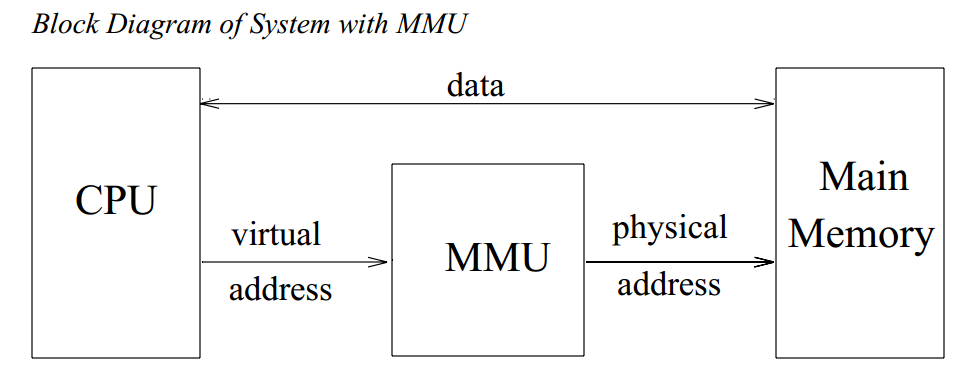
\includegraphics[width=0.7\textwidth]{./figs/block_diagram.png}
	\caption{Block Diagram of MMU}
	\label{fig:example1}
	\end{figure}

The SRMMU supports a fixed 4KB page size and also has support for sparse
address spaces with 3-level map.  A detailed specification of the SRMMU can be
found in Appendix H of the Sparc Architecture Manual.  This document
accompanies a suite of tests for validation of the MMU. The tests are written
in C and Sparc V8 assembly. The tests are organized into three parts :
	\begin{enumerate}
	\item Validation of the basic functionality of the MMU, 
	such as translation and page table walking
	\item Validation of memory protection functionality 
	(checking that correct faults are generated by the MMU
	for all combination of access types and page permissions)
	\item Combined macro-level tests, such as context switching.
	\end{enumerate}
The set of routines used for accessing the MMU registers, performing MMU flush
and probe operations etc.  are given in Appendix \ref{sec:MMU_Access_Routines}.
These routines are common to all tests.




\section{Validation of Basic MMU Functionality}
These tests check the following functionality:
\begin{itemize}
\item Page table reading and address translation
\item Page table walk
\item Context Switching
\item MMU Probe 
\item MMU Flush
\item Enabling and disabling of the MMU
\item Updation of the Referenced bit and Modified bit in a page table entry
\item Functionality of the Cacheable bit in a page table entry
\item Basic trap generation
\end{itemize}  



\subsection{Page Table Reading and Address translation} 
\begin{lstlisting}
(File: ./Page_setup_add_trans/Page_setup_add_trans.c)
\end{lstlisting}

Goal of this test case is to check working of Context Table pointer, Page Set-up and address translation.\\
\textbf{Page Table Set-up} This test program first Disable MMU then stores base address of context table in Context table pointer. Context table contains page tables(Level 1) for respective process. Level  1 page store base address of Level2 Page Table (In PTD format). Similarly Level 2 contains base address of level 3 Page table. Level 3 page table contains PTE.\\
\textbf{Address translation} Test program stores two Test Data to Physical memory such that First data stores at Virtual Address=Physical address and second data stores at physical address where virtual address is mapped.\\
 First it reads data from address from where test Data 1 is stored.But MMU is disabled so VA=PA. It should  read Test Data 1. After this it enables MMU then read from same virtual address. Here it should get Test Data 2.\\
\textbf{Status} \textcolor{blue}{Passed} 

\subsection{Page Table Walk} 
\begin{lstlisting}
(File:./Page_table_walk/Page_table_walk.c)
\end{lstlisting}

Setup page table as explained in Page table setup section.
Then Store PTE of different three pages at each level (1 2 3).\\
Then read/write data from these pages or virtual addresses. If reading/writing is done successfully then Page table walk is working correctly.\\
\textbf{Status} \textcolor{blue}{Passed} 

\subsection{Context Switching}
\begin{lstlisting}
(File:./context_switching/context_switching.c)
\end{lstlisting}

Goal of this Test case is to check context switching in MMU.Context switching is done by switching between page tables.Switching between page tab is done by changing value of context register. 

 It Set-ups two different page table for two different process as described in "Testing of Address translation (Appendix)". It maps logical address X to physical address Y for process 0 and logical address X to physical address Z for process 1.It stores Test data 0 at physical address Y and Test data 1 at physical address Z.
 
Then Test program enable MMU With context register value 0 and read string from logical address X.It should read Test data 0. After this it switches to context 1(How to do context switching is explained in Appendix) and read string from same logical address.It should read Test data 1.\\
\textbf{Status} \textcolor{blue}{Passed}.

\subsection{MMU Probe Functionality} 
\begin{lstlisting}
(File: ./MMU_Probing/MMU_Probing.c)
\end{lstlisting}

Probing mainly used to check PDE and PTE from page directory. In this MMU implementation only probe type 4 is implemented so it always return PTE. Please refer Table H-4 from MMU reference manual. 
How to do probe is explained in Appendix.

\textbf{PTE is not found during probe:}
\begin{lstlisting}
(File: ./MMU_Probing/MMU_Probing_No_PTE.c)
\end{lstlisting}
This test case test error generated by MMU at time probing.
\textbf{Status} \textcolor{blue}{Passed} 

 
\subsection{MMU Flush Functionality} 
\begin{lstlisting}
(File:./mmu_flush/mmu_flush.c)
\end{lstlisting}

This test case mainly check working of MMU flush.Flushing leads to clearing contains of TLB. First it stores two Test data in physical memory at address Y and Z. Test program set-up page table such that logical address X map to physical address Y then it reads data using logical address X. It should read Test data 1.

	Before second read operation it disables MMU and change PTE such that it maps logical address X to Z and then enables MMU.It should read Test data 1 because old PTE is in TLB cache. 

It flushes TLB before 3rd read operation and again read from same logical address. This time it should read Test Data 2, Because TLB contain new updated PTE. \\ \\
Note: ASI for MMU FLUSH PROBE is 0x03.Address doesn't matter here.\\
sta 0x00, [0x00] asi=0x03 ;\\
\textbf{Status} \textcolor{blue}{Passed}.
 
\subsection{Enabling and Disabling of the MMU}
\begin{lstlisting}
(File:./disable_enable/disable_enable.c)
\end{lstlisting}

Goal of this test case is check working of Enable bit (0 th bit) of control register and also testes of address translation from VA to PA before enabling and after enabling MMU.

It set-ups page table as described in "Address translation section"and reads Test Data from virtual address X before enabling MMU. It should read test data 1. Then it enables MMU and read from same virtual address X. It should get Test data 2. Again it disables MMU and Flush Data cache and instruction cache. After this it reads Test Data from same virtual address X. In this should read previous Test Data 1.\\
 \textbf{Status} \textcolor{blue}{Passed}.

\subsection{Updation of the Referenced bit in a Page Table Entry}
\begin{lstlisting}
(File:./modofied_ref_bit/ref/ref_bit_check.c)
\end{lstlisting}
Reference bi is set in PTE(7th bit) when read or write operation occurs on page.
In this case we need to probe MMU and check contains of PTE.
\begin{itemize}
\item Set-up page table as described in " Address translation". 
\item Enable MMU
\item Continue in privilege mode or user mode  and load from given virtual address Ex.0x10000000 
\item Probe MMU at virtual address with type=4 (Please see page 250 for more information in "SPARC V8 Manual"). 
\item To probe use load with alternate space (0x03).
\item Store return value in 32bit integer.
\item Check lower 8 bits.
\end{itemize}
\textbf{Status} \textcolor{blue}{Passed}
 
\subsection{Updation of the Modified bit in a Page Table Entry}
\begin{lstlisting}
(File:./modofied_ref_bit/modified/modofied_bit_check.c)
\end{lstlisting}
Modified bit is set when page contained is modified by user or privilege process.In this case we need to probe MMU and check contain of PTE(6th bit).
\begin{itemize}
\item Set-up page table as described in "Testing of Address translation". 
\item Enable MMU
\item Continue in privilege mode or user mode  and store at given virtual address Ex.0x10000000.
\item Probe MMU at virtual address with type=4 (Please see page 250 for more information in "SPARC V8 Manual"). 
\item To probe uses load with alternate space (0x03).
\item Store return value in 32bit integer.
\item Check lower 8 bits.
\end{itemize}
\textbf{Status} \textcolor{blue}{Passed}

\subsection{Functionality of the Cacheable bit in a Page Table Entry}
\begin{lstlisting}
(File:./cache_bit/cache_bit.c)
\end{lstlisting}
The {\em Cacheable} bit in a PTE specifies if a page should is cacheable or non cacheable.\\
This test program first stores test data 1 at Physical address Y. It maps X to Y and enables MMU with cacheable bit 1. Read data from VA X. It should read test data 1.   
Then it store test data 2 at PA Y using asi=0x20 to 0x2F using MMU bypass. Then again read data from VA X. Again it should read test data 1 instead of test data 2 because test data 1 is in cache.

Then test program stores test data 2 at Physical address Y. It maps X to Y and enables MMU with cacheable bit 0. Read data from VA X. It should read test data 1.   
Then it store test data 2 at PA Y using asi=0x20 to 0x2F using MMU bypass. Then again read data from VA X. But this time it should read test data 2 because data is not in cache.\\
\textbf{Status} \textcolor{blue}{Passed}
\subsection{Traps generated by MMU}
\begin{lstlisting}
(File:./mmu_traps/data_ex_HWtrap09/page_error_HW_trap09.c
 File:./mmu_traps/instr_ex_HWtrap01/page_error_instr_ex_HW01.c)
\end{lstlisting}
Traps are generated by MMU when illegal memory reference take place. Mainly four traps are generated.
\begin{lstlisting}
instruction_access_exception(0x01),data_access_exception(0x09),
instruction_access_MMU_miss,data_access_MMU_miss.
\end{lstlisting}
This test program generate above traps. It has small trap handler at HW0x01 and HW0x09.
It stores trap information in g5 register.\\
Note: Miss traps for both Instruction and Data are not implemented in current MMU design.\\
\textbf{Status} \textcolor{blue}{Passed}
\subsection{Removing entry from TLB when it is Full}
\begin{lstlisting}
(File:./small_TLB/small_TLB.c)
\end{lstlisting}
This test case used to cover lines of source code(MMU.c).
When TLB is full for new entry mmu selects randomly any entry to overwrite. 
For this test case, need to reduce TLB size to 1 from Ajit Hardware Configuration.h. After compiling processor's source file run above test case.

\textbf{Status} \textcolor{blue}{Passed}
\newpage
\section{Validation of Memory Protection by the MMU}

These test cases check memory protection done by MMU. It is expected that MMU should check access permission of  process  with respective page access field. If Process does not have required permission then MMU should generate Fault to protect memory. Information about fault is stored in Fault status register(FSR) and address responsible fault is stored in Fault address register(FAR).
FSR has fields AT(Type of access by process),FT(Fault Type) and L(Page table level where this fault is generated).Also this section tests OW bit,FAV Bit of FSR and No fault bit of MMU control register.\\
\subsubsection{ AT=0 to 7, ACC=xx, Expected FT=1}
\begin{lstlisting}
(File:./AT/ATx/page_error_ATx_Valid_1.c)
\end{lstlisting}
In this case user process try to access memory which is not mapped by OS yet.So there will be no entry for this VA in page tables and MMU will generate Fault type=1 for Access type=0 to 7.\\
Note: x means respective field can have any possible values. 
\begin{lstlisting} 
Ex: ATx => AT0,AT1 to AT7.
\end{lstlisting} 
\begin{itemize}
\item Set-up page table as described in "Testing of Address translation".
\item Enable MMU
\item GO to user mode(Appendix A) or Continue in privilege mode
\item Try to read data or store data or fetch instruction from whose address is not mapped yet in page tables.
\item After this step processor should be go to error state.
\item Check FSR values.
\end{itemize}
\textbf{Status} \textcolor{blue}{Passed}.
\subsubsection{ AT=0, ACC=0 to 3 and 5, Expected FT=0}
\begin{lstlisting}
(File:./AT/AT0/page_error_AT0_S{0 to 3 and 5}.c)
\end{lstlisting}
In this case user process try to access memory which has read access permission to all.

\begin{itemize}
\item Set-up page table as described in "Testing of Address translation".
\item Map 0x10000000 to 0xA0000000 in page table with PTE.ACC=0x86 or 0x86 or 0x8A or 0x8E  or 0x96 .
\item Enable MMU
\item GO to user mode(Appendix A) 
\item Try to read data from 0x10000000.
\item After this step processor should not go to error state.  
\end{itemize}
\textbf{Status} \textcolor{blue}{Passed}.
\subsubsection{ AT=0, ACC=6 and 7, Expected FT=3}
\begin{lstlisting}
(File:./AT/AT0/page_error_AT0_S{6 and 7}.c)
\end{lstlisting}
In this case user process try to access memory which has read access permission for only privilege mode.
This causes privilege violation error.
\begin{itemize}
\item Set-up page table as described in "Testing of Address translation".
\item Map 0x10000000 to 0xA0000000 in page table with PTE.ACC=0x9A or 0x9E .
\item Enable MMU
\item GO to user mode(Appendix A) 
\item Try to read data from 0x10000000.
\item After this step processor should be go to error state. 
\item Check FSR values. 
\end{itemize}
\textbf{Status} \textcolor{blue}{Passed}.
\subsubsection{ AT=0 or 1, ACC=4, Expected FT=2}
\begin{lstlisting}
(File:./AT/AT0or1/page_error_ATx_S4.c)
\end{lstlisting}
In this case privilege process or user process try to read memory which has only execute permission. This causes protection error.

\begin{itemize}
\item Set-up page table as described in "Testing of Address translation".
\item Map 0x10000000 to 0xA0000000 in page table with PTE.ACC=0x92  .
\item Enable MMU
\item GO to user mode(Appendix A) or Continue in privilege mode. 
\item Try to read data from 0x10000000.
\item After this step processor should be go to error state.
\item Check FSR values.
\end{itemize}
\textbf{Status} \textcolor{blue}{Passed}.
\subsubsection{ AT=1, ACC= 0 to 3 and 5 to 7, Expected FT=0}
\begin{lstlisting}
(File:./AT/AT1/page_error_AT1_S{ 0 to 3 and 5 to 7}.c)
\end{lstlisting}
In this case privilege process try to access memory which has read access permission to privilege mode.

\begin{itemize}
\item Set-up page table as described in "Testing of Address translation".
\item Map 0x10000000 to 0xA0000000 in page table with PTE.ACC=0x86 or 0x86 or 0x8A or 0x8E  or 0x96 or 0x9A or 0x9E .
\item Enable MMU 
\item Try to read data from 0x10000000.
\item This process must able to read that data. 
\end{itemize}
\textbf{Status} \textcolor{blue}{Passed}.

\subsubsection{ AT=2, ACC= 2 to 4, Expected FT=0}
\begin{lstlisting}
(File:./AT/AT2/page_error_AT2_S{  2 to 4}.c)
\end{lstlisting}
In this case user process try to execute instruction from memory which has  execute permission to all. 

\begin{itemize}
\item Set-up page table as described in "Testing of Address translation".
\item Map user process instruction space with PTE.ACC=0x8A or 0x8E or 0x92
\item Enable MMU
\item GO to user mode(Appendix A) 
\item Try to execute further instruction.
\item Processor should not go to Error state. 
\end{itemize}
\textbf{Status} \textcolor{blue}{Passed}.
\subsubsection{ AT=2, ACC= 0 to 1 and 5, Expected FT=2}
\begin{lstlisting}
(File:./AT/AT2/page_error_AT2_S{ 0 to 1 and 5}.c)
\end{lstlisting}
In this case user process try to execute instruction from memory which doesn't have  execute permission to user mode or it is not executable memory. This causes protection error.

\begin{itemize}
\item Set-up page table as described in "Testing of Address translation".
\item Map user process instruction space with PTE.ACC=0x82 or 0x86 or 0x96
\item Enable MMU
\item GO to user mode(Appendix A) 
\item Try to execute further instruction.
\item Processor should go to Error state. 
\item Check FSR values.
\end{itemize}
\textbf{Status} \textcolor{blue}{Passed}.
\subsubsection{ AT=2, ACC= 6 to 7, Expected FT=3}
\begin{lstlisting}
(File:./AT/AT2/page_error_AT2_S{6 to 7}.c)
\end{lstlisting}
In this case user process try to execute instruction from memory which doesn't have  execute permission to user mode This causes privilege violation error.

\begin{itemize}
\item Set-up page table as described in "Testing of Address translation".
\item Map user process instruction space with PTE.ACC=0x9E or 0x9A.
\item Enable MMU
\item GO to user mode(Appendix A) 
\item Try to execute further instruction.
\item Processor should go to Error state. 
\item Check FSR values.
\end{itemize}
\textbf{Status} \textcolor{blue}{Passed}.
\subsubsection{ AT=3, ACC= 2 to 4 and 5=6 to 7, Expected FT=0}
\begin{lstlisting}
(File:./AT/AT3/page_error_AT3_S{2 to 4 and 5=6 to 7}.c)
\end{lstlisting}
In this case privilege process try to execute instruction from memory which has  execute permission to all or privilege process. 

\begin{itemize}
\item Set-up page table as described in "Testing of Address translation".
\item Map user process instruction space with PTE.ACC=0x8A or 0x8E or 0x92 or 0x9A or 0x9E. 
\item Enable MMU
\item Continue in privilege mode(Appendix A) 
\item Try to execute further instruction.
\item Processor should not go to Error state. 

\end{itemize}
\textbf{Status} \textcolor{blue}{Passed}
\subsubsection{ AT=3, ACC= 0 to 1 and 5, Expected FT=2}
\begin{lstlisting}
(File:./AT/AT3/page_error_AT3_S{0 to 1 and 5}.c)
\end{lstlisting}
In this case privilege process try to execute instruction from memory which doesn't have execute permission to anyone. This causes protection error.

\begin{itemize}
\item Set-up page table as described in "Testing of Address translation".
\item Map privilege process instruction space with PTE.ACC=0x82, 0x86 and 0x96. 
\item Enable MMU
\item Continue in privilege mode(Appendix A) 
\item Try to execute further instruction. 
\item Processor should go to Error state. 
\item Check FSR values.
\end{itemize}
\textbf{Status} \textcolor{blue}{Passed}
\subsubsection{ AT=4, ACC= 0,2,4 and 5, Expected FT=2}
\begin{lstlisting}
(File:./AT/AT4/page_error_AT4_S{0,2,4 and 5}.c)
\end{lstlisting}
In this case user process try to write memory where user process doesn't have permission to write. This causes protection error.

\begin{itemize}
\item Set-up page table as described in "Testing of Address translation".
\item Map 0x10000000 to 0xA0000000 in page table with PTE.ACC=0x82,0x8A or 0x92  .
\item Enable MMU
\item GO to user mode(Appendix A) 
\item Try to write data to 0x10000000.
\item After this step processor should be go to error state.
\item Check FSR values.
\end{itemize}
\textbf{Status} \textcolor{blue}{Passed}.
\subsubsection{ AT=4, ACC= 6 to and 7, Expected FT=3}
\begin{lstlisting}
(File:./AT/AT4/page_error_AT4_S{6 to and 7}.c)
\end{lstlisting}
In this case user process try to write memory where user process doesn't have permission to write or read or execute. This causes privilege violation error.

\begin{itemize}
\item Set-up page table as described in "Testing of Address translation".
\item Map 0x10000000 to 0xA0000000 in page table with PTE.ACC=0x9A or 0x9E  .
\item Enable MMU
\item GO to user mode(Appendix A) 
\item Try to write data to 0x10000000.
\item After this step processor should be go to error state.
\item Check FSR values.
\end{itemize}
\textbf{Status} \textcolor{blue}{Passed}
\subsubsection{ AT=5, ACC= 0,2,4 and 6, Expected FT=2}
\begin{lstlisting}
(File:./AT/AT5/page_error_AT5_S{0,2,4 and 6}.c)
\end{lstlisting}
In this case privilege process try to write memory where it doesn't have permission to write. This causes protection error.

\begin{itemize}
\item Set-up page table as described in "Testing of Address translation".
\item Map 0x10000000 to 0xA0000000 in page table with PTE.ACC=0x82 or 0x92 or 0x9A.
\item Enable MMU
\item Continue in privilege mode. 
\item Try to write data to 0x10000000.
\item After this step processor should be go to error state.
\item Check FSR values.
\end{itemize}
\textbf{Status} \textcolor{blue}{Passed}
\subsubsection{ AT=6, ACC= 0 to 2 and 4 to 5, Expected FT=2}
\begin{lstlisting}
(File:./AT/AT6/page_error_AT6_S{0 to 2 and 4 to 5}.c)
\end{lstlisting}
In this case privilege process try to write in instruction memory(sta with asi = 0x08) where it doesn't have permission to write. This causes protection error.\\
\textbf{Status} \textcolor{blue}{Passed}

\subsubsection{ AT=6, ACC= 6 to 7, Expected FT=3}
\begin{lstlisting}
(File:./AT/AT6/page_error_AT6_S{6 to 7}.c)
\end{lstlisting}
In this case privilege process try to write in instruction memory(sta with asi = 0x08) where it doesn't have permission to write. This causes privilege violation error.\\
\textbf{Status} \textcolor{blue}{Passed}


\subsubsection{ AT=6, ACC= 3, Expected FT=0}
\begin{lstlisting}
(File:./AT/AT6/page_error_AT6_S{6 to 7}.c)
\end{lstlisting}
In this case privilege process try to write in instruction memory(sta with asi = 0x08) where every one has permission to write. \\
\textbf{Status} \textcolor{blue}{Passed}
\subsubsection{ AT=7, ACC= 0 to 2 and 4 to 6, Expected FT=2}
\begin{lstlisting}
(File:./AT/AT7/page_error_AT7_S{0 to 2 and 4 to 6}.c)
\end{lstlisting}
In this case privilege process try to write in instruction memory(sta with asi = 0x09) where it doesn't have permission to write. This causes protection error.\\
\textbf{Status} \textcolor{blue}{Passed}

\subsubsection{ AT=7, ACC= 3 and 7, Expected FT=0}
\begin{lstlisting}
(File:./AT/AT7/page_error_AT7_S{3 and 7}.c)
\end{lstlisting}
In this case privilege process try to write in instruction memory(sta with asi = 0x09) where every one has permission to write.\\
\textbf{Status} \textcolor{blue}{Passed}

\subsubsection{ FT=4 Translation Error}
\begin{lstlisting}
(File:./FT4/PDE_AT_level3.c)
(File:./FT4/PTE_with_ET3_level0.c)
(File:./FT4/PTE_with_ET3_level1.c)
(File:./FT4/PTE_with_ET3_level2.c)
(File:./FT4/PTE_with_ET3_level3.c)
\end{lstlisting}
A translation error is indicated if an external bus error occurs while the MMU is fetching an entry from a page table, a PTD is found in a level-3 page table, or a PTE has ET=3. It will generate fault type = 4.\\
\textbf{Status} \textcolor{blue}{Passed}

\subsection{PTE is in context table: }
\begin{lstlisting}
(File:./PTE_AT_level0/PTE_AT_level0.c)
\end{lstlisting}
This test case checks address translation of VA when PTE is in context table.\\
\textbf{Status} \textcolor{blue}{Passed}

\subsection{Testing of No Fault Bit}
\begin{lstlisting}
(File:./NF_bit/data_fault/page_error_NF_user_data.c)
(File:./NF_bit/data_fault/page_error_NF_super_data.c)
(File:./NF_bit/instruction/page_error_NF_super_instr.c)
\end{lstlisting}
In this case privilege or user process try to invalid access of memory. 

\begin{itemize}
\item Set-up page table as described in "Testing of Address translation". 
\item Enable MMU and Enable Trap handler
\item Continue in any mode 
\item Try to do invalid access of memory. 
\item Processor should go to Error state. 
\item Check FSR values and FAR.
\item Try again setting No fault bit in control register.
\item End of program check FSR value.
\end{itemize}
\textbf{Status} \textcolor{blue}{Passed}.
\subsection{Testing of OW Flag}
\begin{lstlisting}
(File:./OW_bit/data_fault/page_error_OW_super_data.c)
(File:./OW_bit/data_fault/page_error_OW_user_data.c)
\end{lstlisting}
In this case consecutive  invalid access of memory in User/Supervisor data space causes setting of OW flag.

\begin{itemize}
\item Set-up page table as described in "Testing of Address translation". 
\item Enable MMU and Enable Trap handler
\item Set No fault bit.
\item Continue in any mode 
\item Try to do invalid access of memory more than one.  
\item Check FSR values and FAR.
\end{itemize}
\textbf{Status}\textcolor{blue}{Passed}.


\section{Combined Tests}
\begin{lstlisting}
(File:./large_prog/large_prog.c)
(File:./large_prog/run_large_prog_memmap.txt)

\end{lstlisting}
These test case checks overall functionality of MMU.
This test program have three page tables for three different processes (0,1 and 2). Process 0 and process 1 are mapped at different memory locations. process 0 and process 1 have same subroutine which are mapped to same address space but work differently in both process.
\begin{lstlisting}
To run this test you need to feed  run_large_prog_memmap.txt to
testbech.
\end{lstlisting} 

\newpage
\section{Coverage Report}
Coverage report tells about execution of each line of c-source file. To generate coverage lcov is used. How to generate coverage report is explained in Readme document.\\
\textbf{Result of Coverage Report:}

\begin{tabular}{ |l|l|l| }
  \hline
  Source File & Line coverage & Function coverage\\
  \hline
  Mmu.c & 345/345 (100.0\%) & 20/20 (100.0\%) \\
  \hline
  MmuInterface.c & 24/24 (100.0\%) & 4/4 (100.0\%) \\
  \hline
  StartMmuThreads.c & 21/21 (100.0\%) & 3/3 (100.0\%) \\
  \hline
  TLB.c & 39/39 (100.0\%) & 5/5 (100.0\%) \\
  \hline
\end{tabular}
%\newpage
\section{SPARC Reference MMU Manual's sections covered by Tests:}
\begin{tabular}{ | l |p{5cm}|p{8cm}| }
  \hline
  Sr. No. & Sections & Test Name \\
  \hline
  1. & Section H.3:Page Table Descriptors,Page Table Entry,
  MMU Flush and Probe Model.  & Page table reading and address translation,Page table walk,MMU Probe Functionality,Functionality of the Cacheable bit in a Page Table Entry,MMU Flush Functionality. \\
  \hline
  2. & Section H.4: Control Register,Context Table Pointer
Register,Context Register. & Page Table Reading and Address translation,Context Switching,Enabling and Disabling of the MMU.  \\
  \hline
  3. & Section H.5:Fault Status Register & Validation of Memory Protection by the MMU,Traps generated by MMU,Testing of No Fault Bit,Testing of OW Flag.  \\
  \hline
  4. & Section H.6:Fault Address Register & Validation of Memory Protection by the MMU,Traps generated by MMU .  \\
  \hline
  5. & Section H.7:Referenced and Modified Bit
Updates & Updation of the Referenced bit in a Page Table Entry,Updation of the Modified bit in a Page Table Entry.   \\
  \hline
\end{tabular}




\newpage
\section{Appendix A : MMU Access Routines} \label{sec:MMU_Access_Routines}

The following may be used to embedd assembly code in C :
\begin{lstlisting}
__asm__ __volatile__("AssemblyInstruction");
 \end{lstlisting}
\begin{itemize}
\item \textbf{Set User Mode}
\end{itemize}
By default on reset or power on processor is in privileged mode. 
To go to user mode need to clear S(7th bit) bit from PSR(Processor State Register).

\begin{lstlisting}[language=C]
//---------------Go to user mode--------------------------------
mov %psr, %l0 		!move psr to l0
set 0xFFFFFF7F, %l3	!store 32 bit mask in %l3
and %l0, %l3, %l0 	!clear P(7th bit) using Mask
mov %l0, %psr 		!load l3 in PSR
\end{lstlisting}

\begin{itemize}
\item \textbf{Store values in MMU register}
\end{itemize}
store word mmureg is a function, it is used to write value in MMU register like context table pointer,MMU register control etc. $uint32 t*$ addr this is a passing argument should have address of respective MMU register(Please refer SPARC v8 manual MMU section). This is a privilege instruction and  it should be executed in privilege mode.
\begin{lstlisting}[language=C]
inline void store_word_mmureg(uint32_t value, uint32_t* addr)
{
	__asm__ __volatile__("sta %0, [%1] %2\n\t" : : "r"(value), "r"(addr),
			     "i"(ASI_MMU_REGISTER) : "memory");
}
 \end{lstlisting}

\begin{itemize}
\item \textbf{Read values from MMU register}
\end{itemize}
load word mmureg is a function, it is used to read value from MMU register to in local variable. $uint32 t*$ addr this is a passing argument should have address of respective MMU register(Please refer SPARC v8 manual MMU section).$retval$ return contains of MMU register. This is a privilege instruction and  it should be executed in privilege mode.
\begin{lstlisting}
inline uint32_t load_word_mmureg(uint32_t* addr)
{
 uint32_t retval;
  __asm__ __volatile__("lda [%1] %2, %0\n\t" :"=r"(retval)
 :"r"(addr), "i"(ASI_MMU_REGISTER));
        return retval;
}
 \end{lstlisting}
\newpage
\begin{itemize}
\item \textbf{Flushing of MMU}
\end{itemize}
mmu flush is a function, it is used to flush MMU .Here address doesn't matter. Address and value can be any thing here. Alternate address space should have value 0x3. This is a privilege instruction and  it should be executed in privilege mode.
\begin{lstlisting}
#define ASI_MMU_FLUSH_PROBE	 	0x03
inline void mmu_flush(uint32_t value, uint32_t* addr)
{
__asm__ __volatile__("sta %0, [%1] %2\n\t"  : : "r"(value), "r"(addr), 
	"i"(ASI_MMU_FLUSH_PROBE) : "memory");
}
 \end{lstlisting}

\begin{itemize}
\item \textbf{MMU Probe}
\end{itemize}
mmu probe is a function, it is used to probe MMU . $uint32 t*$ addr this is a passing argument should have address of respective MMU field(Please refer SPARC v8 manual MMU section).$retval$ return contains of MMU register. This is a privilege instruction and  it should be executed in privilege mode.
\begin{lstlisting}
inline uint32_t mmu_probe(uint32_t* addr)
{
uint32_t retval;
__asm__ __volatile__("lda [%1] %2, %0\n\t" :"=r"(retval) : "r"(addr), 
"i"(ASI_MMU_FLUSH_PROBE));
return retval;
}
 \end{lstlisting}

\begin{itemize}
\item \textbf{Flushing of Data and Instruction cache}
\end{itemize}
This function is used for flushing of Data cache and Instruction cache.
\begin{lstlisting}
inline void flush_icache(void)
{
	__asm__ __volatile__(" flush ");
}

//flush_dcache
inline void flush_dcache(void)
{
	__asm__ __volatile__("sta %%g0, [%%g0] %0\n\t" : :
	 "i"(ASI_FLUSH_I_D_CONTEXT) : "memory");
}
 \end{lstlisting}

\newpage
\begin{itemize}
\item \textbf{Context Switching}
\end{itemize}
This function is used for to switch context by changing value of context register. Before changing context register value flushing of Both cache is required.
\begin{lstlisting}
//context switch.
//make a switch to a particular context
inline void context_switch(uint32_t context_number)
{
	//flush dcache
	//putString("\nflush dcache");
	__asm__ __volatile__("sta %%g0, [%%g0] %0\n\t" : :
	"i"(ASI_FLUSH_I_D_CONTEXT) : "memory");
	//flush icache
	//putString("\nflush icache");
	__asm__ __volatile__(" flush ");
	//flush TLB
	//putString("\nflush TLB");
	__asm__ __volatile__("sta %%g0, [%%g0] %0\n\t"  : :
	 "i"(ASI_MMU_FLUSH_PROBE) : "memory");

	//write new context number into mmu context register
	//putString("\nnew context number");
	__asm__ __volatile__("sta %0, [%1] %2\n\t" : :
	 "r"(context_number), "r"(MMU_REG_CONTEXT),
			     "i"(ASI_MMU_REGISTER) : "memory");

	//putString("\nflush dcache");
	//flush dcache
	__asm__ __volatile__("sta %%g0, [%%g0] %0\n\t" : :
			     "i"(ASI_FLUSH_I_D_CONTEXT) : "memory");
	//flush icache
	//putString("\nflush icache");
	__asm__ __volatile__(" flush ");
	//flush TLB
	//putString("\nflush TLB");
	__asm__ __volatile__("sta %%g0, [%%g0] %0\n\t"  : :
	 "i"(ASI_MMU_FLUSH_PROBE) : "memory");


}
 \end{lstlisting}
\newpage
\begin{itemize}
\item \textbf{Setting up Page tables}
\end{itemize}
This section discus about how to set page tables.Fist we need to set global variables.As shown below
\begin{lstlisting}
//Context table
uint32_t ContextTable[256]  __attribute__((aligned(0x1000)));
//Page tables for process 1:
uint32_t process1_L1PageTable[256] __attribute__((aligned(0x1000)));
uint32_t process1_L2PageTable[64]  __attribute__((aligned(0x1000)));
uint32_t process1_L3PageTable[64]  __attribute__((aligned(0x1000)));
//Page tables for process 2:
uint32_t process2_L1PageTable[256] __attribute__((aligned(0x1000)));
uint32_t process2_L2PageTable[64]  __attribute__((aligned(0x1000)));
uint32_t process2_L3PageTable[64]  __attribute__((aligned(0x1000)));
 \end{lstlisting}
 
Declare one pointer which will point to base of context table. Address value should be store in PTD(Page Table descriptor ) format.
Ex: 
\begin{lstlisting}
	uint32_t context_table_ptr_value 
 \end{lstlisting}
Then store contain of above pointer in MMU's context table pointer.
\begin{lstlisting}
#define MMU_REG_CONTEXT_TABLE_PTR	0x00000100
store_word_mmureg(context_table_ptr_value,
 (uint32_t*)MMU_REG_CONTEXT_TABLE_PTR);
 \end{lstlisting}
 
Make all entry of context table is invalid by writing zeros.Then store Base Address of process1's level1 page table in context[0] location in PTD format. Similarly for process2.
Similarly base address of level2 page table in Level 1 page table entries for respective process.
PTE can be at any page level.
PTE format is as described in SPARC V8 manual. Higher 24 bit of PTE contains Bits of 35 to 13 of physical address.Lower 8 bit describe different properties of pages like access,read,write permission.   
\begin{lstlisting}
	for(i=0xD0; i<=0xFF; i++)
	{
	//PTE feilds : USER ASI:(Instruction=0x8,Data=0xA)
	 SUPER ASI:(Instruction=0x9,Data=0xB)
	// C M R ACC ET
	// 1 0 0 000 10 = 0x82 user:Read_only Super:Read_only.
	// 1 0 0 001 10 = 0x86 user:Read_only/Write
	 Super:Read_only/Write.
	// 1 0 0 010 10 = 0x8A user:Read_only/Execute
	 Super:Read_only/Execute.
	// 1 0 0 011 10 = 0x8E user:Read_only/Write/Execute
	 Super:Read_only/Write/Execute.
	// 1 0 0 100 10 = 0x92 user:Execute_only
	 Super:Execute_only.
	// 1 0 0 101 10 = 0x96 user:Read_only Super:Read/Write.
	// 1 0 0 110 10 = 0x9A user:No Acess.
 Super:Read/Execute.
	// 1 0 0 111 10 = 0x9E user:No Acess. Super:Read/Write/Execute.
		uint32_t PPN = (i<<12);
		uint32_t PTE_level1 = (PPN<<8) | (0x8E);//In this any 
		one can read/write/ execute
		uint32_t PTE_level2 = (PPN<<8) | (0x9A);//In this contex 
		only supervisor can execute
		process1_L1PageTable[i] = PTE_level1;
		process2_L1PageTable[i] = PTE_level2;
	}
 \end{lstlisting}
 
\begin{itemize}
\item \textbf{Enable or Disable MMU}
\end{itemize} 
To enable MMU need to set 0th bit of MMU register control. Whose address is 0x0.
 \begin{lstlisting}
#define MMU_REG_CONTROL			0x00000000
	//----------------------MMU Enable---------------------------------------
	uint32_t MMU_control_word = 0x1; //set the Enable bit
	store_word_mmureg(0x0, (uint32_t*) MMU_REG_CONTEXT);//Enable 
	with 0th context.
	store_word_mmureg(MMU_control_word, (uint32_t*)
	 MMU_REG_CONTROL);
);
//----------------------MMU Disable---------------------------------------
uint32_t MMU_control_word = 0x0; //Clear Enable bit
 store_word_mmureg(MMU_control_word, (uint32_t*) MMU_REG_CONTROL);
);
 \end{lstlisting}
 
 
\section{Appendix B : The Fault Status Register Fields}

\begin{figure}[h]
\centering
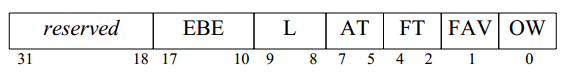
\includegraphics[width=12cm]{./figs/FSR.png}
\caption{FSR Register}
\label{fig:example2_1}
\end{figure}


Whenever there is invalid access of memory MMU generates signal to CPU and update it's Fault status register. FAR stores address of VA memory that was responsible for Fault.
FSR(Fault status register(32 bit)) has 6 different fields.

\textbf{EBE}  Bits in the External Bus Error field are set when a system error occurs
during a memory access. The meanings of the individual bits are
implementation-dependent. Examples of system errors are: timeout,
uncorrectable error, and parity error. The MMU need not implement all
the bits in EBE. Unimplemented bits read as zeros.
 
 \textbf{L}
  The Level field is set to the page table level of the entry which caused the
fault. If an external bus error is encountered while fetching a PTE or
PTD, the Level field records the page table level of the page table containing the entry.
The Level field is defined as follows:
\begin{figure}[h]
\centering
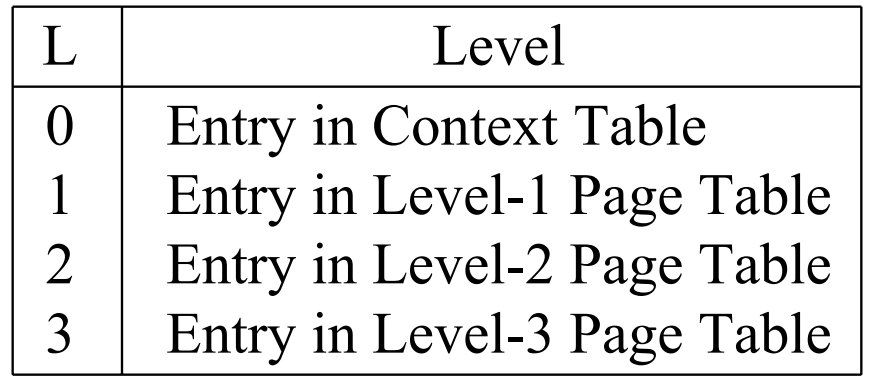
\includegraphics[width=6cm]{./figs/level_FSR.png}
\caption{FSR Register}
\label{fig:level_FSR}
\end{figure}

 \textbf{AT} The Access Type field defines the type of access which caused the fault.
(Loads and stores to user/supervisor instruction space can be caused by
load/store alternate instructions with ASI = 8 or 9). The AT field is defined as follows:
\begin{figure}[h]
\centering
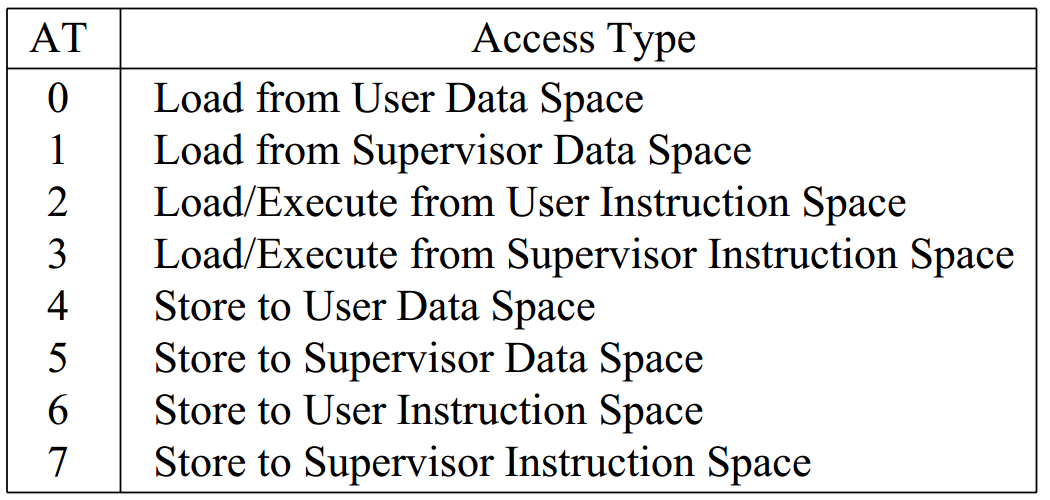
\includegraphics[width=8cm]{./figs/AT.png}
\caption{FSR Register}
\label{fig:AT}
\end{figure}

\textbf{FT}The Fault Type field defines the type of the current fault. It is defined as follows:
\begin{figure}[h]
\centering
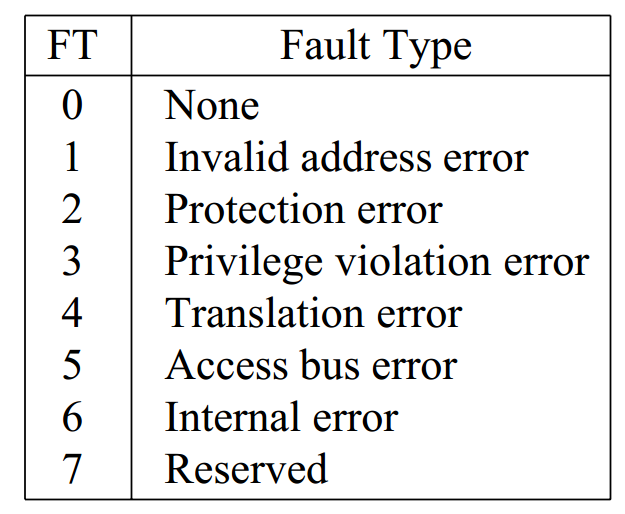
\includegraphics[width=6cm]{./figs/FT.png}
\caption{FSR Register}
\label{fig:AT}
\end{figure}

\newpage
Invalid address, protection, and privilege violation errors depend on the Access
Type field of the Fault Status Register and the ACC field of the corresponding
PTE. The errors are set as follows:
\begin{figure}[h]
\centering
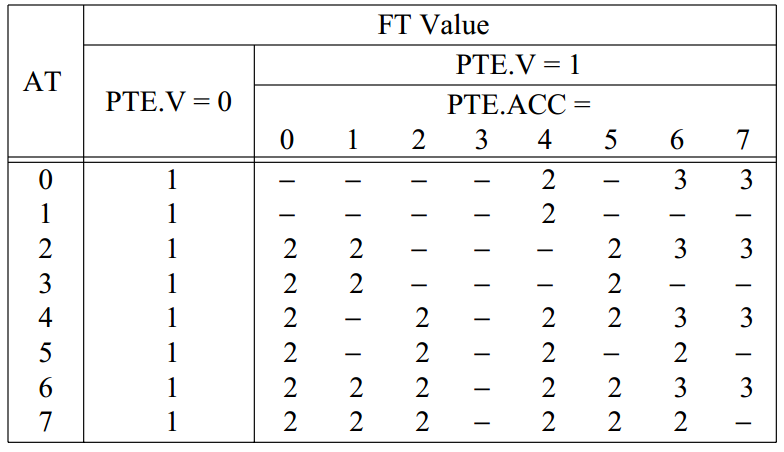
\includegraphics[width=10cm]{./figs/AT_FT.png}
\caption{}
\label{fig:AT_FT}
\end{figure}

\textbf{FAV}The Fault Address Valid bit is set to one if the contents of the Fault
Address Register are valid. The Fault Address Register need not be valid
for instruction faults. The Fault Address Register must be valid for data
faults and translation errors.

\textbf{OW}
The Overwrite bit is set to one if the Fault Status Register has been written more than once by faults of the same class since the last time it was
read. If an instruction access fault occurs and the OW bit is set, system software must determine the cause by probing the MMU and/or memory. 
 
%\part{Introduction}
%\section{Installing Latex}
%\subsection{MMU }
%\begin{center}
%\end{center}
%$$(x_2+1)$$  

\end{document}
